\section{Metodología Experimental}
\subsection{Polarizador Lineal}
Nuestro primer objetivo fue identificar la polarización de un láser rojo \qty{632}{\nm} de longitud de onda, haciéndolo incidir sobre un polarizador lineal que fue rotado 36 veces, para obtener una separación angular de \ang{5} entre medición, y midiendo la potencia transmitida con un potenciómetro.
Si el láser estaba polarizado linealmente, entonces al rotar el polarizador lineal observaríamos un comportamiento obediente a la ley de Malus \eqref{eq: Malus}. En cambio, si la luz tiene una polarización circular o no está polarizada mediremos una potencia constante.

\subsection{Retardador de Fase}

Posteriormente, colocamos entre la fuente y el polarizador lineal un retardador de media longitud de onda con su eje rápido inclinado a \ang{30} respecto a la vertical, como se muestra en la figura \ref{fig: labo}.
\begin{figure}[H]
    \centering
    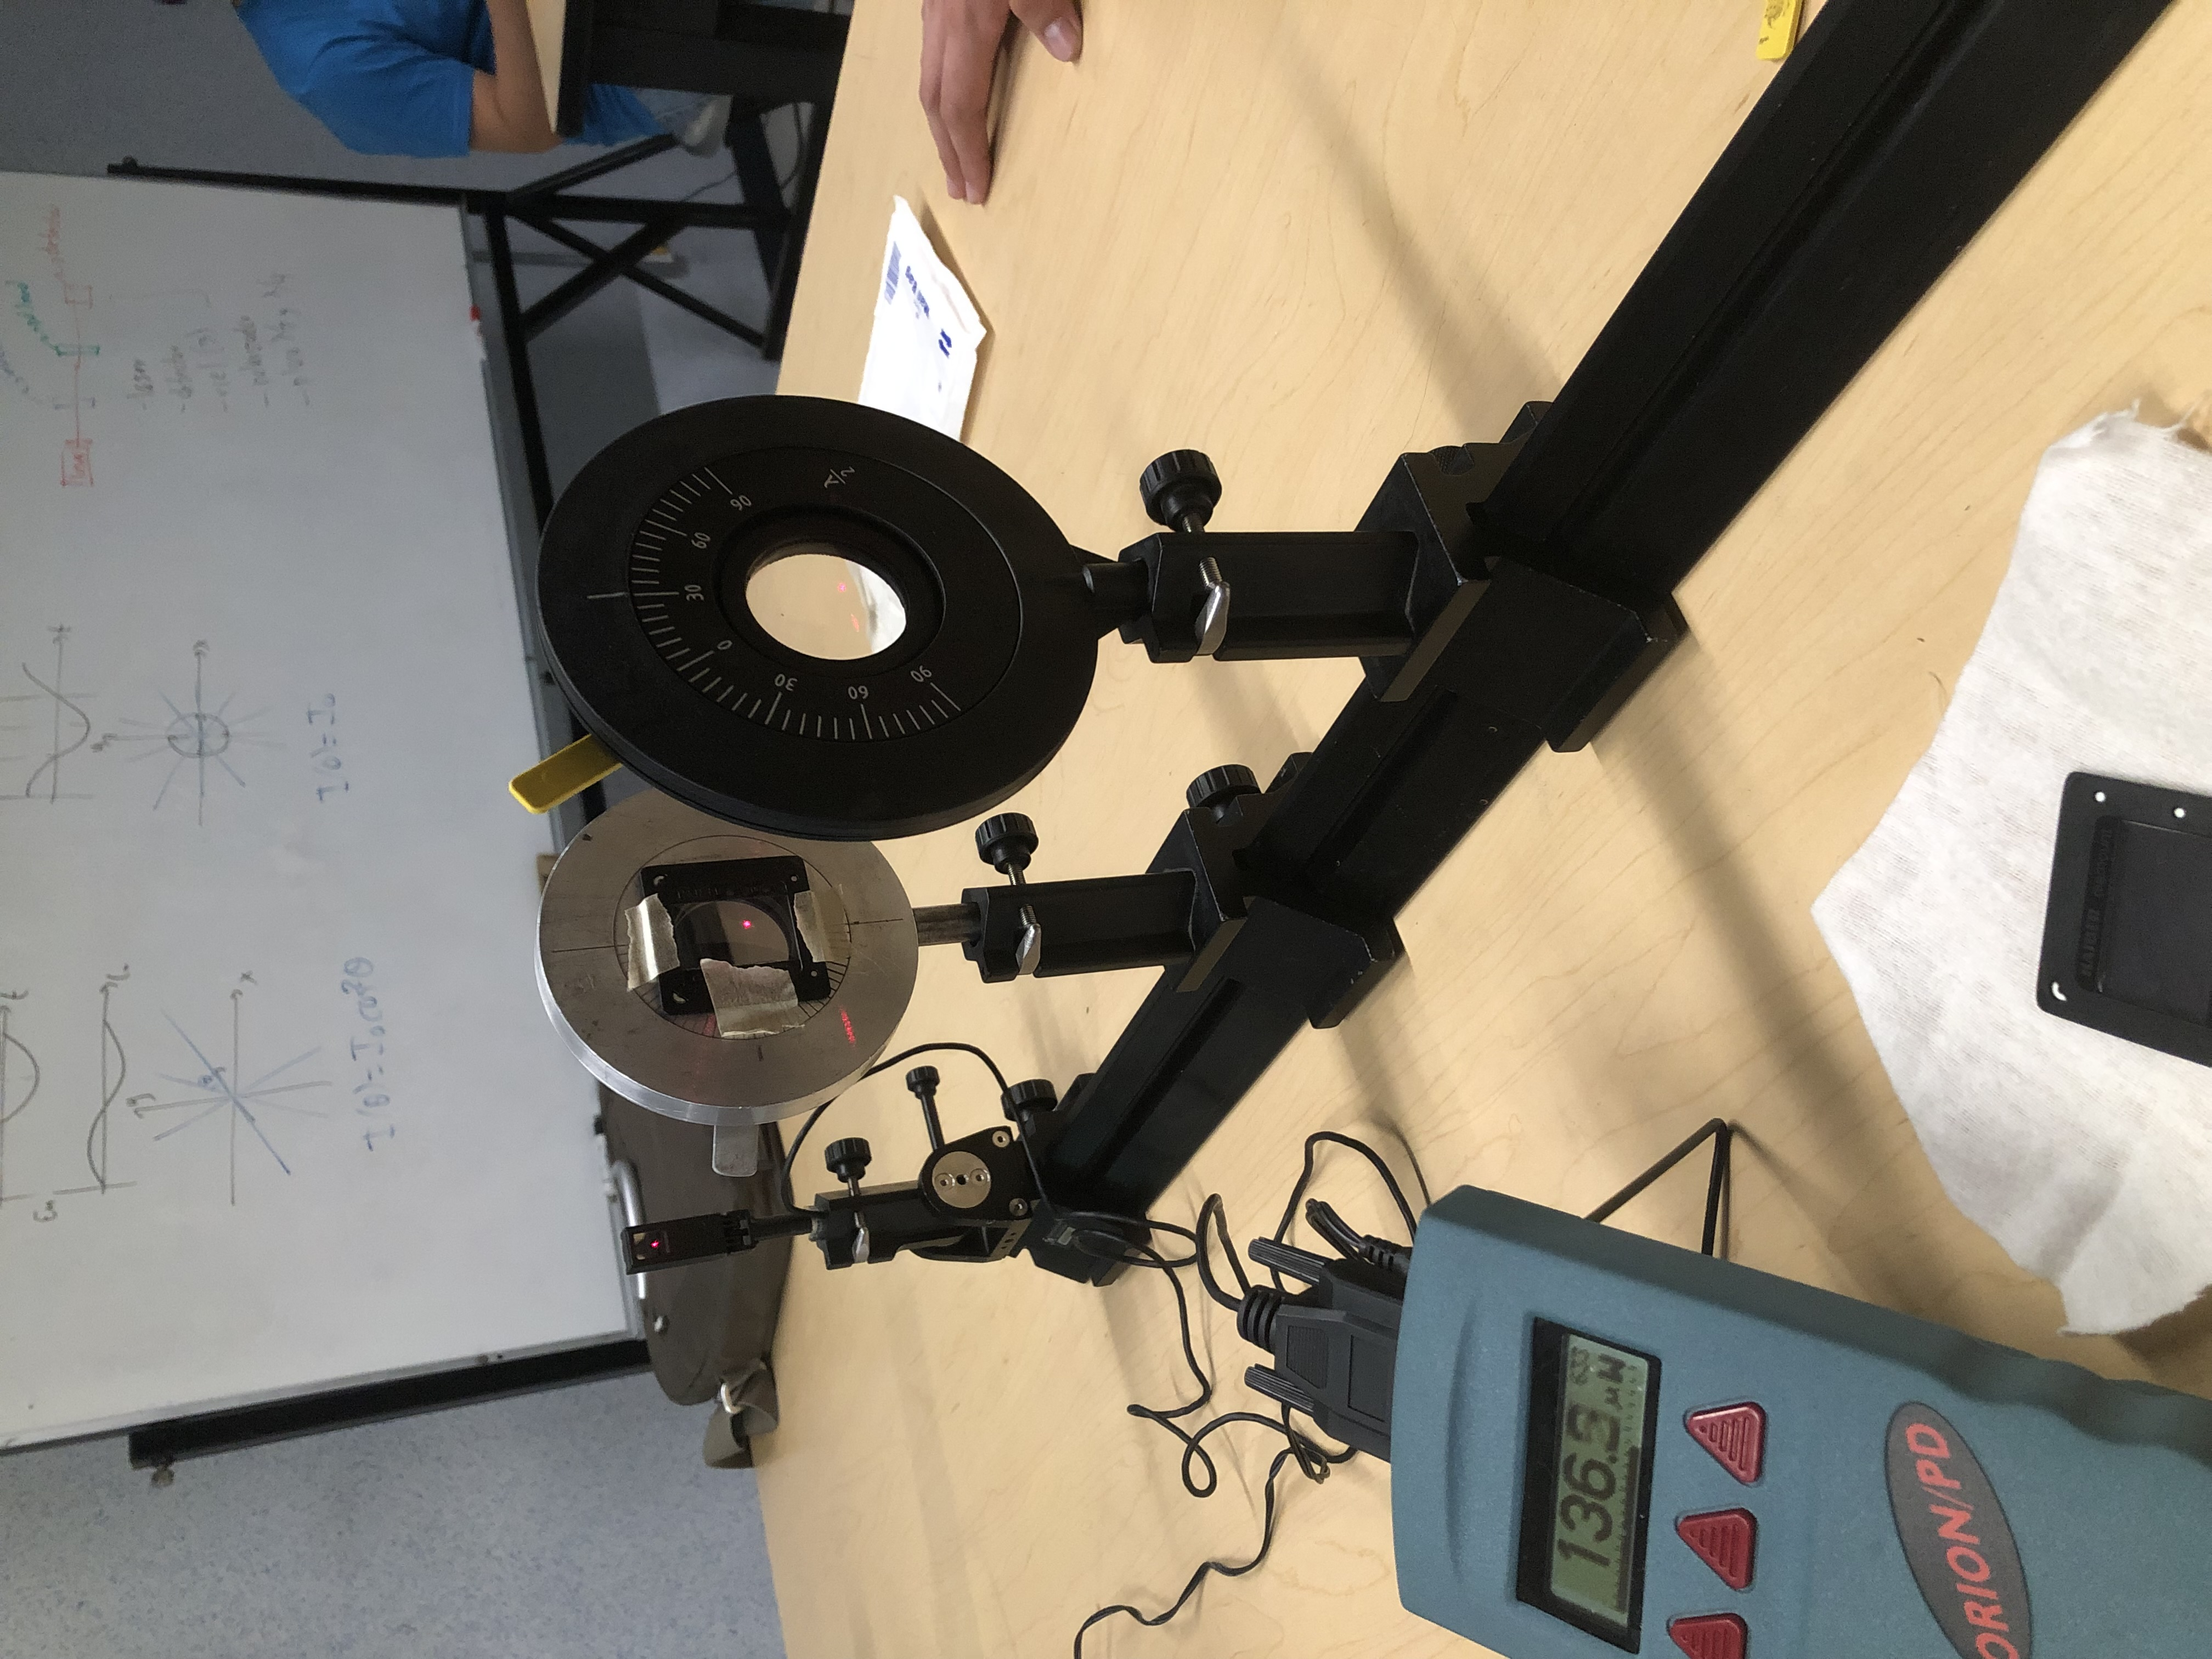
\includegraphics[width=0.9\linewidth, angle=-90]{Imagenes/labo.jpeg}
    \caption{Antes de incidir sobre el polarizador lineal (disco plateado), se introduce una diferencia de fases en el láser con un retardador de fase (disco negro).}
    \label{fig: labo}
\end{figure}

Posteriormente reemplazamos el retardador de $\lambda/2$ por uno de $\lambda/4$ con su eje rápido a \ang{45} y repetimos las 36 mediciones. Finalmente repetimos las mediciones con el retardador de un cuarto de longitud de onda a \ang{-50}.